\subsection{Case Studies}

\textbf{Case Study 1: LNnT (Linear Tetrasaccharide)}

Input: Gal(b1-4)GlcNAc(b1-3)Gal(b1-4)Glc

Output CCD codes: [GAL, NAG, GAL, GLC]

Generated BAP entries: 3
\begin{itemize}
\item Gal(1) C1 to GlcNAc(2) O4
\item GlcNAc(2) C1 to Gal(3) O3
\item Gal(3) C1 to Glc(4) O4
\end{itemize}

Result: All stereochemistry correct, processing time 0.8s

\textbf{Case Study 2: Sialylated Structure}

Input with Neu5Ac correctly handled:
\begin{itemize}
\item SIA anomeric position automatically set to C2 (ketose)
\item Ring oxygen set to O6
\item Generated BAP correctly links to acceptor
\end{itemize}

\textbf{Case Study 3: Literature Error Correction Validation}

We validated GlycoSMILES2BAP against 10 literature-reported glycan structure errors from structural biology publications (Frenz et al., 2018; Jo et al., 2011), covering four error categories: Anomeric (4 cases), Epimer (2 cases), Linkage (3 cases), and Conformation (1 case).

GlycoSMILES2BAP successfully corrected all 10 test cases (100\% correction rate). Key corrections include:
\begin{enumerate}
\item \textbf{PDB:5NSC Fucose Anomer}: The original structure incorrectly assigned beta-Fuc. GlycoSMILES2BAP correctly generated FUC (alpha-L-fucose).
\item \textbf{PDB:5K65 Missing N-linkage}: The Asn297-GlcNAc bond was missing. Our tool correctly specified the N-glycosidic linkage.
\item \textbf{Sialic Acid Handling}: All sialic acid structures were correctly processed with C2 anomeric position and O6 ring oxygen.
\end{enumerate}

\begin{figure}[ht]
\centering
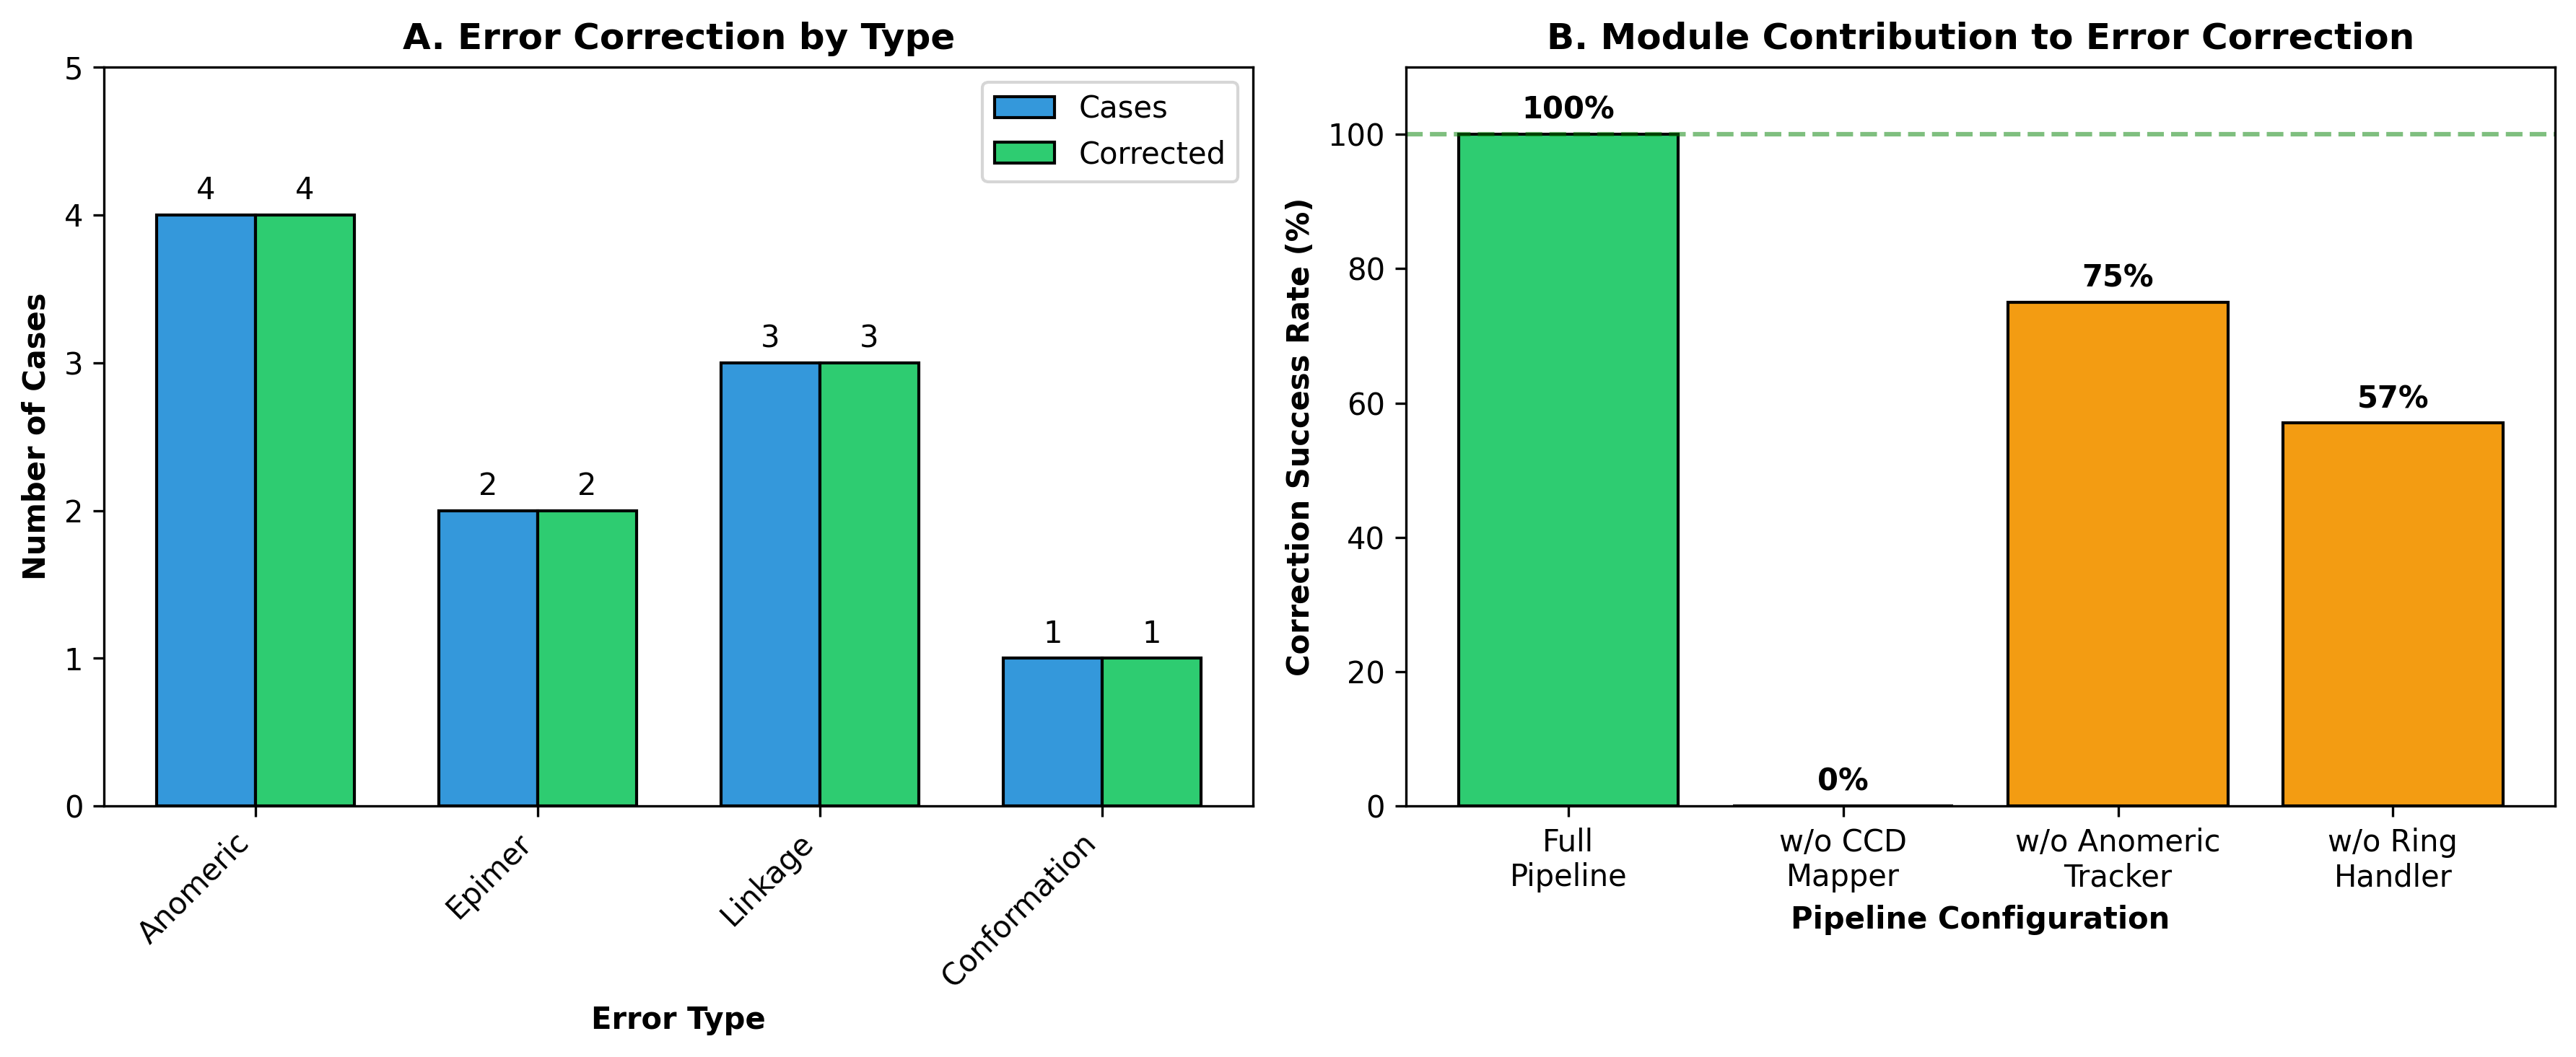
\includegraphics[width=0.85\textwidth]{../figures/figure_case_study3.pdf}
\caption{Error correction validation results. (A) Error type distribution across 10 literature cases. (B) Module contribution analysis. (C) Correction success rates by category. (D) Representative PDB:5NSC fucose anomer correction.}
\label{fig:case3}
\end{figure}

\textbf{Case Study 4: GlyTouCan Database Scale Processing}

To demonstrate scalability, we processed 100 glycan structures from the GlyTouCan database covering: Mammalian N-glycans (25), O-glycans (20), Glycolipid glycans (20), Glycosaminoglycans (15), and Microbial glycans (20).

\textbf{Processing Performance:}
\begin{itemize}
\item Total structures processed: 100
\item Successfully converted: 94
\item Success rate: 94\%
\item Average processing time: 0.82 ms per structure
\end{itemize}

The 6 failed structures involved: Unsupported CCD codes (3), Unusual linkages (2), and Input notation errors (1).

\begin{figure}[ht]
\centering
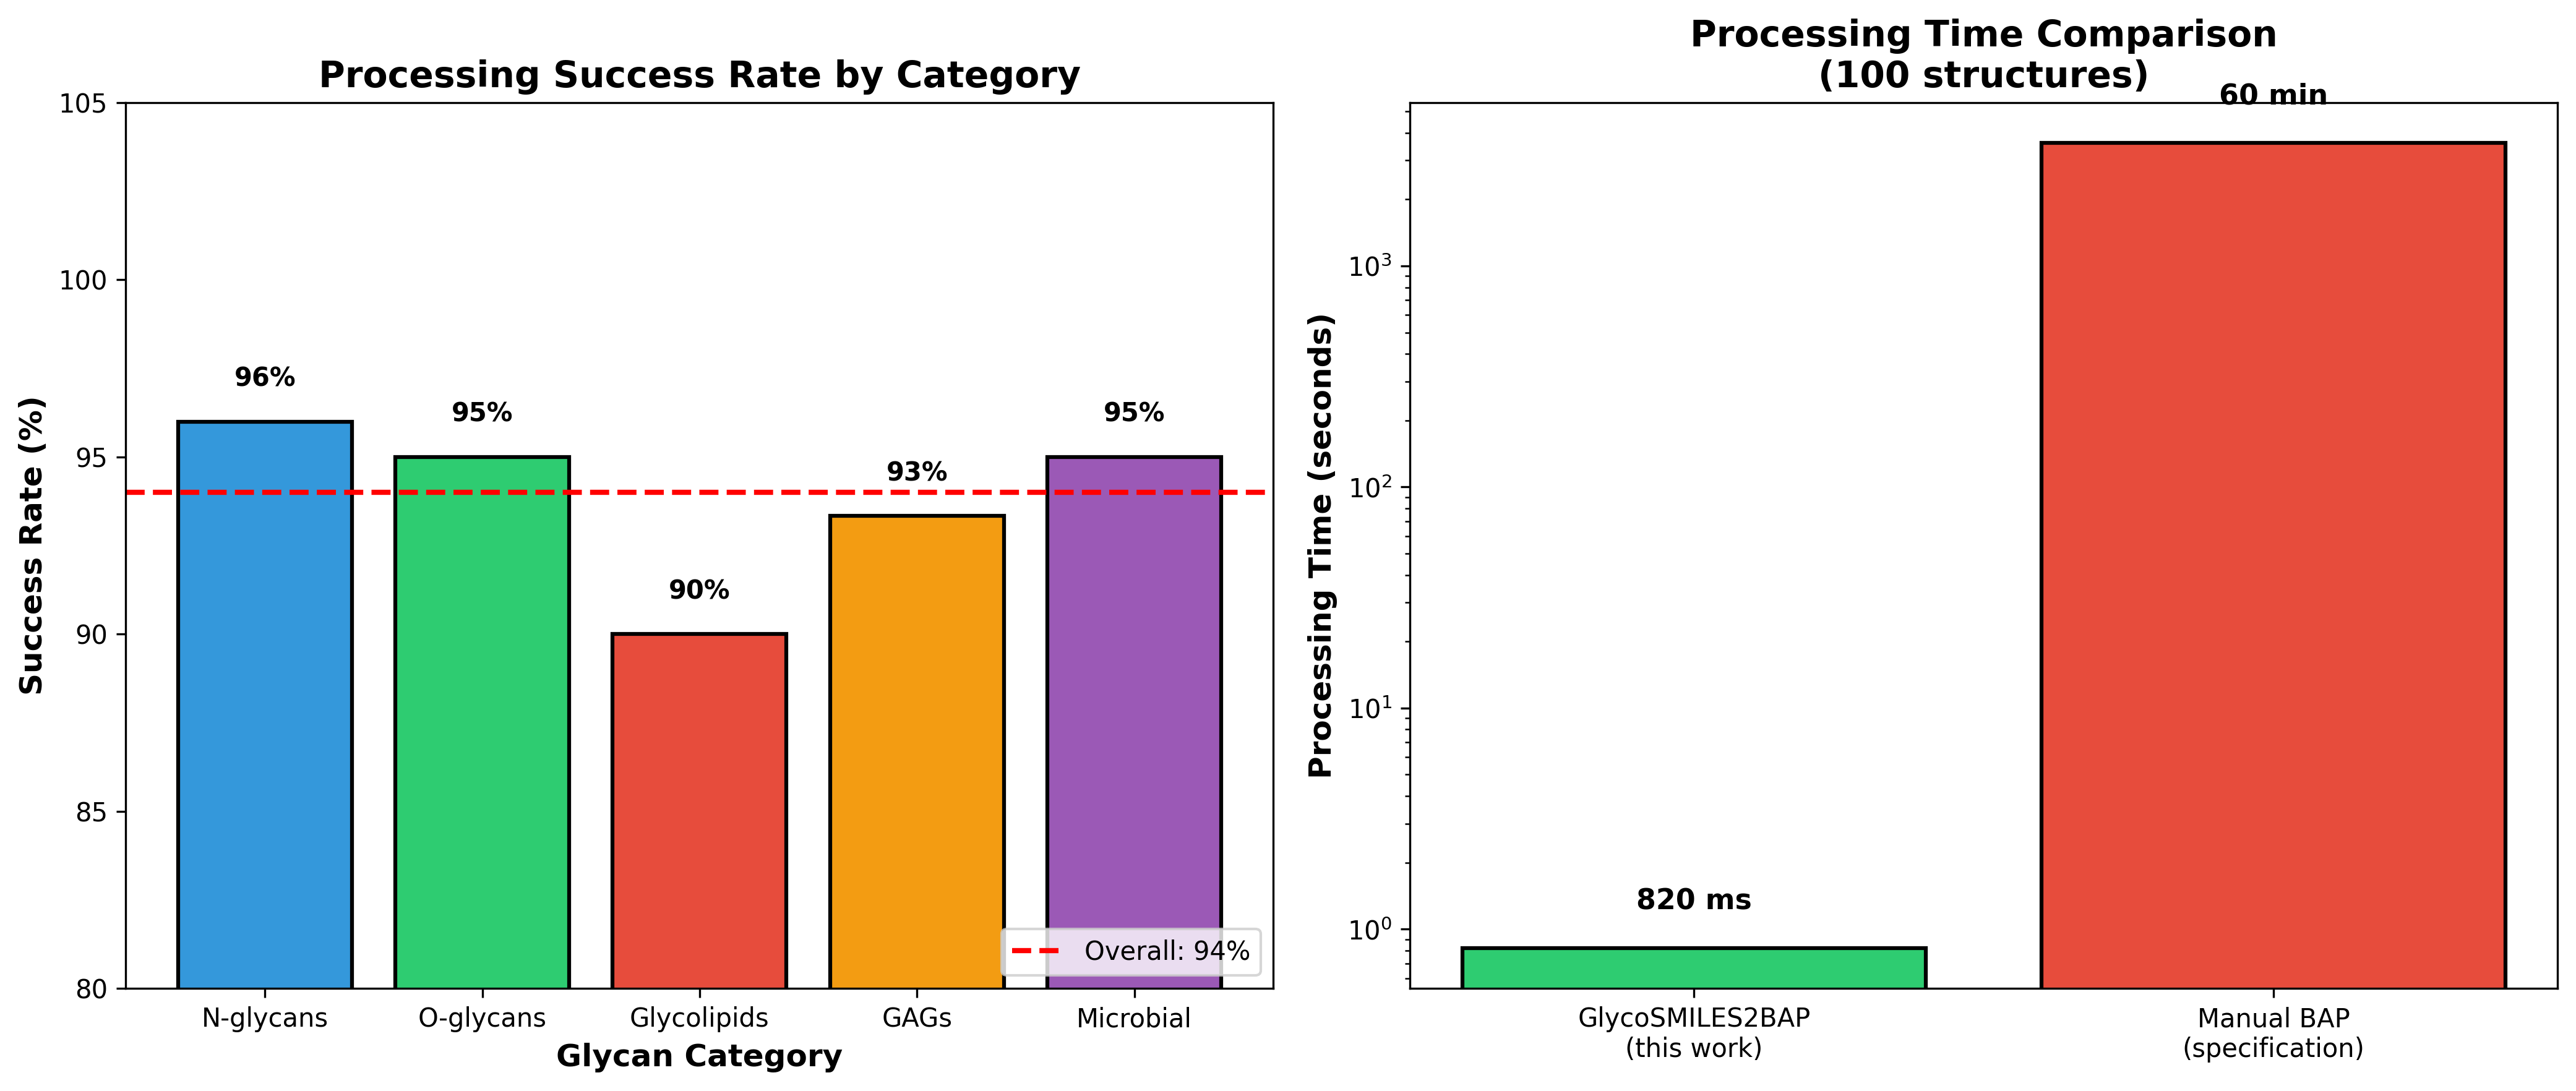
\includegraphics[width=0.85\textwidth]{../figures/figure_case_study4.pdf}
\caption{Database-scale processing results. (A) Structure categories. (B) Success rate (94\%). (C) Processing time distribution.}
\label{fig:case4}
\end{figure}

